\section{Introduction}
The jobs ecosystem in LinkedIn powers the career needs of 450 Million plus
professionals around the world. The two-main means of finding a job via
LinkedIn are through search and recommendations. Traditional information
retrieval involves matching and scoring a set of documents given query.
Personalized search involves scoring documents given query and {\bf user}~\cite{liget}.  
Both search and recommendations pose unique set of constraints on quality and
latency.

LinkedIn job search and recommendations are used in different parts of the
ecosystem with different types of constraints. 
Figures~\ref{fig:jymbii-jobs-home} and~\ref{fig:jymbii-in-feed} show the
use case for jobs recommendations in LinkedIn jobs home and LinkedIn feed (home
page) respectively.
The LinkedIn
feed~\cite{agarwal2015personalizing} personalizes the experience by merging
different sources of information including posts, comments, news articles and
jobs. Each of these sources (including job recommendations) must respond with
very tight SLAs (Service Level Agreements, usually latency constraints imposed
by the callers of a service) for the home page or the app to be responsive.
In job recommendations, there is no explicit query to filter the results.
The underlying recommendations model is deeply personalized with per member and
per job coefficients. Such personalization helps us achieve very high
relevancy~\cite{zhang2016glmix}. Scoring all possible jobs for each member in
this complex model would be prohibitively expensive and will certainly not meet
our SLA requirements. At the same time, scoring very few documents would result
in loss of relevance. 

Job search has similar issues as well. While search has an explicit query,
sometimes the query can be way too broad (example: {\it marketing}).
These broad queries match several millions of jobs and ranking all of them
would not meet our latency requirements.
There are several such head queries ({\it marketing, sales}) which exhibit
similar characteristics.
In this case, we
could leverage information in the member's profile to bias the query towards
jobs he/she may be interested in.

One common way of handling too many matching documents is to pass through
multiple levels of ranking layers. The ranking layer closest to the retrieval stage is coarse
and biases it's decision towards recall and not precision. But, as we move to
higher levels, we move on to more complex ranking functions which take more time, but
also, rank fewer documents. In this regard, we generally separate out the
search/recommendations flow into two steps pre-retrieval and post retrieval.
Pre-retrieval involves constructing the query based on both the explicit query
from user as well as personalization added on top of it and post retrieval
involves going through multiple layers of ranking. The post retrieval ranking
for both search and recommendations is well studied~\cite{liu2009learning}. 

The objective of query construction is to formulate a query to our retrieval
engine such that we minimize the number of documents ranked (direct impact on
latency) while making sure we score the relevance documents. In this work, we
propose a decision tree based approach towards query construction that meets the
aforementioned objective. The key contribution of the work includes: 
\begin{enumerate}
        \item We convert the query construction problem into a decision tree
            problem with branches in the tree corresponding to query clauses 
            and show that such a formulation scales for very large number of features. 
            We show that such a formulation can have a huge impact on latency
            without affecting quality of the results - {\bf all at LinkedIn scale.}
        \item We developed an offline replay mechanism which does a true
            evaluation of the underlying ranking metric while evaluating reduction
            in latency. It also increases the experimentation velocity by near
            accurate reproduction of production behavior and reduces number of
            A/B tests needed with live traffic. 
        \item The framework is generic across search and recommendations so
            long as the underlying retrieval is based on an inverted index.
\end{enumerate}
The techniques described in this work are all in production. In job search it
resulted in p99 (worst 1\% of the queries) latency reduction of {\bf 67\%} 
and in jobs recommendations, we show a p99 latency reduction of {\bf 55.96\%}. While
p99 queries are more important on an operational perspective, we also show
significant reduction in latency for median case as well. While we did not
explicitly target quality metrics, we did find a {\bf 3.5\%} improvement in job
application as a result of this approach. We attribute this improvement mainly
due to reduction in timeouts to our callers (due to improved latency). All
results shown were obtained by online A/B testing. {\bf As of writing this paper, 
the techniques described in this work power all of job search and
recommendations at LinkedIn.}


\begin{figure}
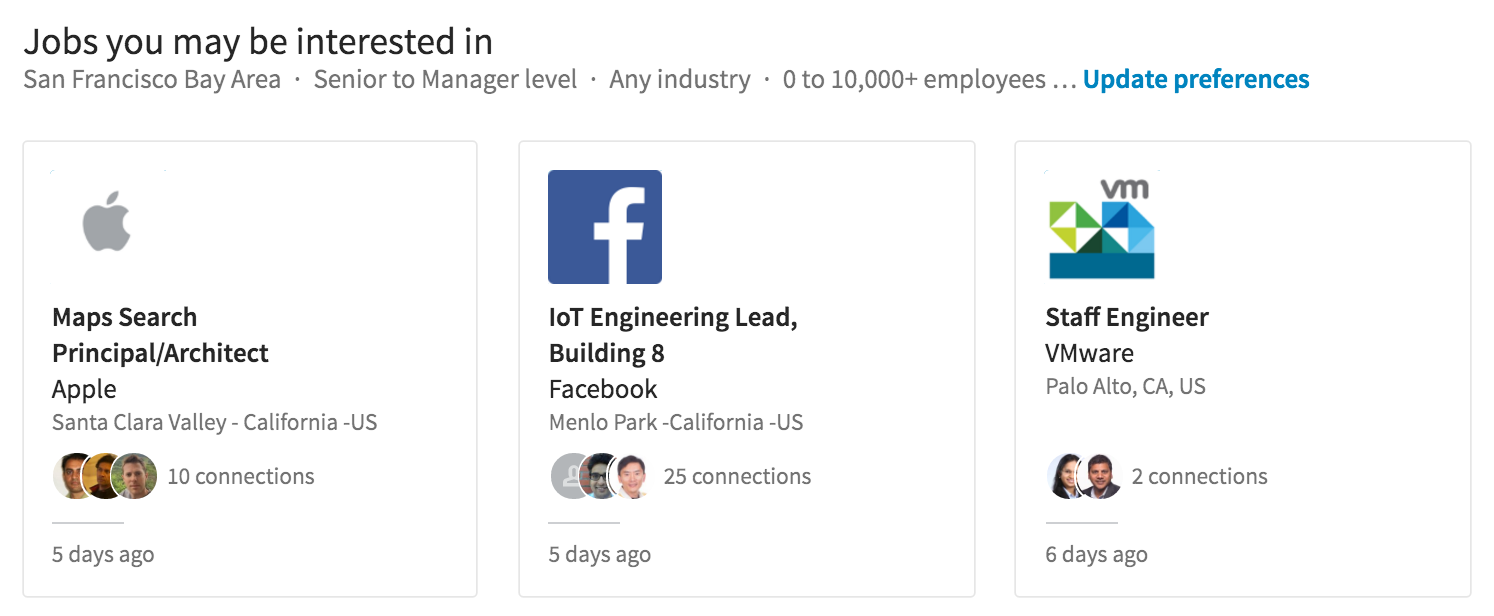
\includegraphics[width=\linewidth,height=\textheight,keepaspectratio]{jymbii.png}
\caption{Jobs recommendations in jobs homepage}
\label{fig:jymbii-jobs-home}
\end{figure}

\begin{figure}

\includegraphics[width=\linewidth,height=\textheight,keepaspectratio]{jymbii-in-feed.png}
\caption{Jobs recommendations in LinkedIn feed}
\label{fig:jymbii-in-feed}
\end{figure}
